\documentclass[tikz, border=10pt]{standalone}
\usepackage{tikz}
\usetikzlibrary{shapes.geometric, arrows.meta, positioning, shadows}
\begin{document}
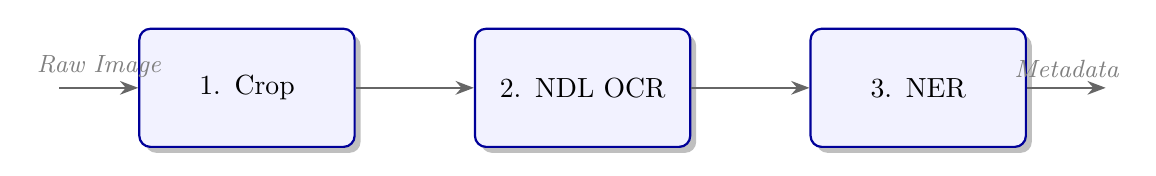
\begin{tikzpicture}[
    node distance=1.5cm,
    auto,
    process/.style={
        rectangle, draw=blue!60!black, fill=blue!5, thick,
        text width=2.5cm, align=center, rounded corners,
        minimum height=1.5cm, drop shadow
    },
    arrow/.style={thick, ->, >=Stealth, color=gray!80!black},
    label/.style={font=\small\itshape, color=gray}
]
    % Nodes
    \node (step1) [process] {1. Crop};
    \node (step2) [process, right=of step1] {2. NDL OCR};
    \node (step3) [process, right=of step2] {3. NER};
    % Connections
    \draw [arrow] (step1) -- (step2);
    \draw [arrow] (step2) -- (step3);
    % Labels
    \draw [arrow] ([xshift=-1cm]step1.west) -- (step1) node[midway, above, label] {Raw Image};
    \draw [arrow] (step3) -- ([xshift=1cm]step3.east) node[midway, above, label] {Metadata};
\end{tikzpicture}
\end{document}
